\graphicspath{{sec00/images/}{sec00/code/}}
\lstset{inputpath=sec00/code/}

%%%%%% предыстория лекция Смаля
\begin{frame}{Предыстория}\relax
    \centering
    
\includegraphics[width=0.9\linewidth]{prevLaTeX}
    % В 2015 году была лекция ``LaTeX: краткое введение в качественную типографику'' от Александра Владимировича Смаля
    
    % \cscfootnote{aaaa}
    \cscfootnote{\url{https://compscicenter.ru/videos/latex/}}
     
\end{frame}

\outclassframe{
\begin{frame}{Предыстория}\relax
    \begin{itemize}
        \item В 2015 году в CSC была лекция ``LaTeX: краткое введение в качественную типографику'' от Александра Владимировича Смаля
        \item Она знакомила с основами \LaTeX\ и показывала прелесть этой системы
        \item Если вы видите эти строки в записи и лишь начинаете изучать \LaTeX, советую ознакомиться с лекцией
        \item И прочитать книгу Львовского ``набор и верстка в системе \LaTeX''
    \end{itemize}
    
    
    \cscfootnote{\url{https://compscicenter.ru/videos/latex/}}
     
\end{frame}
}

\begin{frame}{\LaTeX\ vs Power Point}\relax
    \begin{itemize}
        \item Для большинства задач -- дело вкуса
        \item Написание в \LaTeX\ обычно медленнее
        \item В \LaTeX\ гораздо проще делать ``по правилам'', единообразно
        \item В \LaTeX\ есть больше свободы в создании необычных фич. Хотя это свобода редко нужна.
        \begin{itemize}
            \item Но по ходу лекции вы, надеюсь, будете замечать вещи, которые было бы проблематично сделать в Power Point
        \end{itemize}
         
    \end{itemize}
     
\end{frame}

\begin{frame}{\LaTeX\ vs \TeX}\relax
    \begin{enumerate}
        \item {\ccsc\TeX - подход}. Использование тех команд и макросов, которые вшиты в \TeX, созданный Доннальдом Кнутом начиная с 1978 г
        \item {\ccsc\LaTeX - подход}. Использование расширения \TeX 'а, созданное Лесли Лэмпортом. (версия $2\epsilon$ появилась в 1994 г)
        \item {\ccsc package\LaTeX - подход}. Использование команд из расширений \LaTeX'а разной степени стандартности
    \end{enumerate}
     
     Особое внимание будем уделять первому подходу как базовому.
     
\end{frame}

\begin{frame}{Что сегодня узнаем?}\relax
    \begin{enumerate}
        \item Примитивы в \LaTeX
        \begin{enumerate}
            \item Как \TeX\ видит наш документ: боксы и клей
            \item Какие примитивы существуют: длины, счётчики и другое
            \item Как манипулировать примитивами
        \end{enumerate}
        
        \item Программирование в \TeX\ и \LaTeX
        \begin{enumerate}
            \item Создание макросов
            \item Условные операторы
            \item Циклы и рекурсия
            \item Операции ввода-вывода
            \item Отладка
        \end{enumerate}
         
    \end{enumerate}
    \inpause Эта лекция для тех, кто уже знает \LaTeX\ хотя бы на уровне книги Львовского
\end{frame}


\begin{frame}{Для чего вам эти знания}\relax
    \moveleft1.4cm\hbox{\vbox{
     \begin{description}
         \item[\textbf{{\huge-}}]~
         \begin{itemize}
              \item Скорее всего не понадобится
              \item Документы можно составлять и из готовых шаблонов
         \end{itemize}\pause
         \item[\textbf{{\huge+}}]~
         \begin{itemize}
              \item Для общей эрудиции
              \item ``подправлять'' используемые шаблоны 
              \item писать свои шаблоны
              \item автоматизировать работу
         \end{itemize}
     \end{description}
     }}
\end{frame}


\begin{frame}{Обо мне}\relax
     \begin{itemize}
         \item закончил CSC в 2015 году
         \item стажировался в Papeeria, онлайн \LaTeX -редакторе
         \item младший научный сотрудник в Сколковском институте науки и технологий
          
     \end{itemize}
\end{frame}

{\supressfootnotefalse
\begin{frame}{Некоторые соглашения}{Сноски}\relax
    
    \cscfootnote{Как эта}
    \begin{itemize}
         \item Для повторного прочтения
         \item Некоторые детали по работе с командами
         \item Ссылки на источники
         \item Комментарии
         \item будут видны вне класса
    \end{itemize}
\end{frame}
}

\begin{frame}{Некоторые соглашения}{``магические'' слайды}\relax
Слайды с дополнительной информацией
\magicPage

\begin{itemize}
     \item Для полноты картины
     \item Но не для анализа в классе
\end{itemize}
\end{frame}

{\renewcommand{\inclass}[1]{#1}\renewcommand{\outclass}[1]{#1}
\inclassframe{
\begin{frame}{Некоторые соглашения}{Слайды только для класса}\relax
     Такие слайды исчезнут в выкладываемой лекции.~\\~\\

    \inclasshigh{Так обозначаем сноску, которая будет только в классе видна}
\end{frame}
}
\outclassframe{
\begin{frame}{Некоторые соглашения}{Слайды только для чтения}\relax
    Такие слайды появятся в выкладываемой лекции.~\\~\\

    \outclasshigh{Так обозначаем сноску, которая будет только вне классе видна}
\end{frame}
}
}

\begin{frame}{Задача -- сделать шаблон выступлений}\relax
    Наша практическая задача сегодня-- реализовать шаблон, с которым я рассказываю =)
    \begin{itemize}
        \item номера страниц и логотип
        \item возможность писать сноски 
        \item работа с заголовком
        \item прогрессбар
    \end{itemize}
    
    \outclasshigh{\textit{примечание:} моя задача -- проиллюстрировать основные идеи. Не везде предлагаемое решение будет State~of~the~Art, где-то будет немного костылей. Но будет работать}
    
\end{frame}
%% 7-8 минут по сюда

%% start point
% \outclassframe{
% \begin{frame}{Начнём с пустого шаблона}\relax
%      \centering
%     \fbox{
\includegraphics[width=0.9\linewidth]{01_init}}
%     \outclass{\cscfootnote{см папку ``01\_init''}}
% \end{frame}
% }

\lookCode{Сделаем простой файл презентации}

%%%%%%%%%%%%%%%%%%%%%%%%%%%%%%%%% создание команд 
\section{Слегка продвинутый \LaTeX: Типографика и создание команд}
\subsection{Простое создание команд}


\begin{frame}{Где пишем код}\relax
     Код можно писать 
     \begin{itemize}
         \item Прям в начале документа
         \item Внутри \{\} (будет локален)
         \item В классах
         \item В стилевых файлах
     \end{itemize}
     \outclass{На уровне языка отличий класса от стиля нет. Концептуальное различие: класс это нечто глобальное, стили могут подходить к разным классам.}
\end{frame}


\begin{frame}[fragile]{Создание команд}\relax
    
    % \lstset
    % {
    %     basicstyle=\tt\normalsize,
    % }
    \footnotesize
     \begin{tabbing}
     
        \lstinline|\newcommand{|\= \lstinline|\mycommand| \= \lstinline|[1]|  \=  \lstinline|{something #1}|\kill

        \rulecommand{1}\lstinline|\newcommand{|\> \rulecommand{2}\lstinline|\mycommand}| \> \rulecommand{3}\lstinline|[1]|  \>  \rulecommand{4}\lstinline|{something #1}| \\ \footnotesize
        создаём команду\>  \>   \>  \\ 
        \>\footnotesize имя команды \>   \>  \\ 
        \>  \>\footnotesize число аргументов (может  отсутствовать)  \>  \\
        \>  \>  \>\footnotesize тело \\
    \end{tabbing}
    
    \cprotect\outclasshigh{\lstinline|\renewcommand| чтобы пересоздать}
\end{frame}

\lookCode{Создадим команду для быстрого набора ``Computer Science Center''.\par Пишем \ccol\CSC, получаем ``Computer Science Center''
\begin{enumerate}
    \item Запишем команду в .tex файл 
    \item Создадим пакет -- файл стилей  .sty 
    \item Перенесём команду в пакет 
     
\end{enumerate}
}

% \cprotect\outclassframe{
\begin{frame}[fragile]{Начало .cls и .sty файлов}\relax
     Класс:
     \begin{lstlisting}
     \NeedsTeXFormat{LaTeX2e}
     \ProvidesClass{<class-name>}[<date in YYYY/MM/DD> <other info>]
     \end{lstlisting}
     
     Стиль:
     \begin{lstlisting}
     \NeedsTeXFormat{LaTeX2e}
     \ProvidesPackage{<package-name>}[<date in YYYY/MM/DD> <other info>]
     \end{lstlisting}
     
     
     \cscfootnote{\lmanc{3.3.1}[19] \normalfont\url{https://www.latex-project.org/help/documentation/clsguide.pdf}}
    
\end{frame}
% }

\begin{frame}{Специальный синтаксис внутри пакетов}\relax
    Внутри пакетов синтаксис меняется:

    {\centering
    \begin{tabular}{rcl}
         \ccol\newcommand& $\to$ & \ccol\providecommand\\
         \ccol\usepackage & $\to$ & \ccol\RequirePackage\\
         \ccol\documentclass & $\to$ & \ccol\LoadClass
    \end{tabular}}
    ~\\~\\ 
        

    \inclasshigh{\pause Обратите внимание на нотацию двух последних команд}

    \inpause
    \outclasshigh{происходят дополнительные проверки на отсутствие дублирования}

\end{frame}

\lookCode{Изменим создание команду создания команды \ccol\CSC\ на \ccol\providecommand,\\ Создадим новую команду, выделяющую текстовый фрагмент по цвету {\ccsc Вот так вот}\pause
\begin{enumerate}
    \item Подключим пакет для работы с цветами
    \item Определим нужные цвета 
    \item Создадим команду работы с цветом
     
\end{enumerate}
\pause

Вопрос: как сделать линейку сверху слайда? (Как прогрессбар)
}

% %%%%%%%%%%%%%%%%%%%%%%%%%%%%%%%%%%%%%%%%%%%%%%%% Длины %%%%%%%%%%%%%%%%%%%%%%

\subsection{Длины: единицы измерения}
\def\showLength#1{
    \raise4pt\hbox{%
        \vrule height 6pt depth 2pt%
        \highgreen{\rule{#1}{4pt}}%
        \vrule height 6pt depth 2pt%
    } 
    #1
}

\begin{frame}{Длины}{абсолютные значения}\relax

    \centering
    чаще всего используется:
    
    \begin{tabular}{r|cc|l}
         pt& points & $\simeq$0.35mm & \showLength{12pt} \\
         mm& millimeters & $\simeq$2.84pt & \showLength{10mm} \\
         cm& centimeter & $\simeq$28.4pt, 10mm & \showLength{1cm} \\
         in& inch & $\simeq$72.27pt, 25.4mm  & \showLength{1in} \\
    \end{tabular}
    
    
    \cscfootnote{\wikiC{https://en.wikibooks.org/wiki/LaTeX/Lengths} \knuthc{10}[68] \lvoc{I.2.10}[26]}
\end{frame}


\begin{frame}[fragile]{Длины}{Относительные значения}\relax
    
    \centering
    
    
    \begin{tabular}{r|c|l}
        %  pt& points  & \showLength{12pt} \\
        %  mm& millimeters & \showLength{10mm} \\\hline
         em& примерно \highgreen{ширина} буквы \highgreen{'M'} & \showLength{1em} \\
         ex& примерно \highgreen{высота} буквы \highgreen{'x'} & \showLength{1ex} \\\hline
    \end{tabular}
    
    \inpause пример: если добавим команду \verb|\Huge|
    
    \begin{tabular}{r|l}
         mm & \showLength{5mm} \\
         em & \showLength{1em} \\\hline
         \Huge mm & \Huge \showLength{5mm} \\
         \Huge em & \Huge \showLength{1em} \\
    \end{tabular}
    
    % use {\ccsc em} for horizontal and {\ccsc ex} for vertical cases
    
    \cscfootnote{\wikiC{https://en.wikibooks.org/wiki/LaTeX/Lengths} \knuthc{10}[68] \lvoc{I.2.10}[26]}
\end{frame}

\cprotect\outclassframe{
\begin{frame}[fragile]{Предзаданные длины}{Наиболее используемые}\relax

\centering
\begin{tabular}{r|l}
    \multicolumn{2}{c}{\tiny\TeX's}\\\hline
     \ccol\parindent & Размер отступа в параграфе\\
     \ccol\parskip & \footnotesize Вертикальный отступ для нового параграфа \\
     \hline\multicolumn{2}{c}{\tiny\LaTeX's}\\\hline
     \ccol\textwidth & Ширина текста на странице\\
     \ccol\textheight & Высота текста на странице\\
     \ccol\linewidth & Ширина текста в ``боксе''\\
     \ccol\lineheight & Высота текста в ``боксе''\\
\end{tabular}

     \cscfootnote{\wikiC{https://en.wikibooks.org/wiki/LaTeX/Lengths\#LaTeX_default_lengths} \lmanc{5.5}[34] \stExC{https://tex.stackexchange.com/questions/16942/difference-between-textwidth-linewidth-and-hsize}\\ 
     \ccol\parskip\ на самом деле это клей}
\end{frame}
}

% \cprotect\outclassframe{
\begin{frame}[fragile]{Арифметика с длинами}\relax
    \lstset
    {
        basicstyle=\tt\normalsize,
    }
    \begin{itemize}
        \item Можно домножать как \lstinline|0.5\textwidth|
        \item Нельзя просто так использовать +, -, *, /
        \begin{itemize}
            \item Это можно сделать с помощью команды \ccol\dimexpr: \lstinline|\dimexpr\textwidth - 30pt|
        \end{itemize}
    \end{itemize}

    \cscfootnote{\stExC{https://tex.stackexchange.com/questions/245635/formal-syntax-rules-of-dimexpr-numexpr-glueexpr}}
\end{frame}
% }

\lookCode{Пустим по верху линейку как в прогрессбаре 
\begin{enumerate}
    \item Модифицируем \texttt{headline}
    \item Сделаем ведущий цвет зелёным
    \item Используем линейку нужной длины командой \ccol\rule
     
\end{enumerate}
}
\lookCode{...И по низу пустим лого, заметки и отображение страниц 

{\centering
\includegraphics[width=0.7\textwidth]{05_footnote.png}\par}
\pause
\begin{enumerate}
     \item Модифицируем \texttt{footnline}
     \item Перенесём файл логотипа в рабочую папку
     \item добавим логотип с помощью \ccol\includegraphics
     \item добавим номер слайда с \ccol\insertframenumber
     \item Создадим команду для добавления заметки
\end{enumerate}

\pause 

Вопрос: Как сделать, чтобы длинные заметки не уводили номер страницы за экран?}


%%%%%%%%%%%%%%%%%%% boxes и glue (счётчик лишь слегка)

\subsection{Боксы и клей}
\begin{frame}{Основная идея \TeX а}\relax
    \centering \large
    \tabcolsep=0.15em
    \begin{tabular}{r>{\ccsc}l}
         Символ -- это & бокс\\
         он -- часть слова, которое & бокс\\ 
         слова соединены & клеем\\ 
         в предложения и параграфы.&\\ 
         Параграф, кстати, это & бокс\\
         он соединён с другими & клеем\\
         в страницу. Которая -- & бокс\\
         &\\ 
         таблица, картинки, ... -- это & бокс 
    \end{tabular}
    
    \cscfootnote{\wikiC{https://en.wikibooks.org/wiki/LaTeX/Boxes} \knuthc{11}[73]}
\end{frame}


\begin{frame}{Параметры бокса: высота, глубина, ширина}
     
    \centering
    \newbox\boxtodimen%
    \newdimen\hb%
    \newdimen\db%
    \newdimen\wb%
    
    \setbox\boxtodimen=\hbox{\fontsize{120}{126}\selectfont y}%
    \hb=\ht\boxtodimen%
    \db=\dp\boxtodimen%
    \wb=\wd\boxtodimen%
    
    \newcommand{\boxingDimF}{%
    \leavevmode 
    
    \hbox to \wb{%
        \hbox to 0pt{\box\boxtodimen}%
        \hbox to 0pt{\vbox to 0pt{\hbox{%
            \leavevmode 
            \hbox to 0pt{\raisebox{0pt}[0pt][0pt]{\color{green!40!black}\rule{\wb}{1.7pt}}}%width
            \hbox to 0pt{\raisebox{0pt}[0pt][0pt]{\rule{\wb}{0.4pt}}}%width2
            \hbox to 0pt{\raisebox{0pt}[0pt][0pt]{\color{red}\rule{1.7pt}{\hb}}}%height
            \hbox to 0pt{\raisebox{-\db}[0pt][0pt]{\color{red!40!yellow}\rule{1.7pt}{\db}}}%depth
        }}}%
        \hbox to 0pt{\vbox to 0pt{\hbox{%
            \hbox to 0pt{\raisebox{-\db}[0pt][0pt]{\rule{0.4pt}{\dimexpr\hb+\db}}}%left
            \hbox to 0pt{\hbox to \wb{}\raisebox{-\db}[0pt][0pt]{\rule{0.4pt}{\dimexpr\hb+\db}}}%right
            \hbox to 0pt{\raisebox{\hb}[0pt][0pt]{\rule{\wb}{0.4pt}}}%top
            \hbox to 0pt{\raisebox{-\db}[0pt][0pt]{\rule{\wb}{0.4pt}}}%bottom
        }}}%
    }%
    }
    
    \centering
    \begin{tikzpicture}
        \inclass{\uncover<1>}{\node at (0.5\wb, 0) {\raisebox{\hb}{\fontsize{120}{126}\selectfont y}};}
         \inclass{\uncover<2,3>}{\node at (0.5\wb, 0) {\raisebox{\hb}{\boxingDimF}};}
         \inclass{\uncover<3>}{\fill(0,0) circle (0.1cm);
         \node(rp) at (0,0) {};
         \node(rpt) at (-6em, 0) {reference point};
         \draw[->] (rpt) -- (rp);
         \node(bl) at (\wb+8em, 0) {base line};
         \draw (\wb,0) -- (bl);
         
         \node(wdth) at (0.5\wb, -\db-1.4ex) {\color{green!40!black}width};
         \draw[<-] (0, -\db-1.4ex) -- (wdth);
         \draw[->] (wdth) -- (\wb, -\db-1.4ex);
         \draw (0, -\db) -- +(0, -2.8ex);
         \draw (\wb, -\db) -- +(0, -2.8ex);
         
         \node(dpth) at (\wb+1.6em, -0.5\db) {\color{red!40!yellow}depth};
         \draw[<-] (\wb+1.6em, 0) -- (dpth.north);
         \draw[->] (dpth.south) -- (\wb+1.6em, -\db);
         \draw (\wb, -\db) -- +(3.2em, 0);
    
         \node(hght) at (\wb+1.6em, +0.5\hb) {\color{red}height};
         \draw[<-] (\wb+1.6em, 0) -- (hght.south);
         \draw[->] (hght.north) -- (\wb+1.6em, \hb);
         \draw (\wb, \hb) -- +(3.2em, 0);}
    \end{tikzpicture}
     
     \cscfootnote{\stExC{https://tex.stackexchange.com/questions/40977/confused-with-tex-terminology-height-depth-width}}
\end{frame}

    \newcommand{\boxingDim}[1]{{%
    \ifcsname boxtodimen\endcsname%
    \else%
    \newbox\boxtodimen%
    \newdimen\hb%
    \newdimen\db%
    \newdimen\wb%
    \fi%
    \leavevmode 
    \setbox\boxtodimen=\hbox{#1}%
    \hb=\the\ht\boxtodimen%
    \db=\the\dp\boxtodimen%
    \wb=\the\wd\boxtodimen%
    \hbox to \wb{%
        \hbox to 0pt{\box\boxtodimen}%
        \hbox to 0pt{\vbox to 0pt{\hbox{%
            \leavevmode 
            \hbox to 0pt{\raisebox{0pt}[0pt][0pt]{\color{green!40!black}\rule{\wb}{1.7pt}}}%width
            \hbox to 0pt{\raisebox{0pt}[0pt][0pt]{\rule{\wb}{0.4pt}}}%width2
            \hbox to 0pt{\raisebox{0pt}[0pt][0pt]{\color{red}\rule{1.7pt}{\hb}}}%height
            \hbox to 0pt{\raisebox{-\db}[0pt][0pt]{\color{red!40!yellow}\rule{1.7pt}{\db}}}%depth
        }}}%
        \hbox to 0pt{\vbox to 0pt{\hbox{%
            \hbox to 0pt{\raisebox{-\db}[0pt][0pt]{\rule{0.4pt}{\dimexpr\hb+\db}}}%left
            \hbox to 0pt{\hbox to \wb{}\raisebox{-\db}[0pt][0pt]{\rule{0.4pt}{\dimexpr\hb+\db}}}%right
            \hbox to 0pt{\raisebox{\hb}[0pt][0pt]{\rule{\wb}{0.4pt}}}%top
            \hbox to 0pt{\raisebox{-\db}[0pt][0pt]{\rule{\wb}{0.4pt}}}%bottom
        }}}%
    }%
    }%
    }
\begin{frame}{Как \TeX\ объединяет боксы}
    
    \inclass{{\centering
    % \boxingDim{
    \only<1,2,3>{\leavevmode\hbox{\fontsize{120}{126}\selectfont\boxingDim{{g}}\inpause\boxingDim{f}\inpause\boxingDim{\textit{y}}\boxingDim{\textit{:}}\boxingDim{.}}}
    % }
    \only<4>{\boxingDim{{\fontsize{120}{126}\selectfont\boxingDim{{g}}\inpause\boxingDim{f}\inpause\boxingDim{\textit{y}}\boxingDim{\textit{:}}\boxingDim{.}}}}

    }}
    \outclass{{\centering
    % \boxingDim{
    % {\leavevmode\hbox{\fontsize{120}{126}\selectfont\boxingDim{{g}}\inpause\boxingDim{f}\inpause\boxingDim{\textit{y}}\boxingDim{\textit{:}}\boxingDim{.}}}
    % }
    {\boxingDim{{\fontsize{120}{126}\selectfont\boxingDim{{g}}\inpause\boxingDim{f}\inpause\boxingDim{\textit{y}}\boxingDim{\textit{:}}\boxingDim{.}}}}

    }}

    \outclasshigh{Обратите внимание, что бокс не совпадает полностью с буквой. ``f'' выходит за неё, точка занимает не всё пространство бокса}

\end{frame}

\begin{frame}{Два типа боксов}\relax
     
    Есть два типа боксов:
    \begin{itemize}
        \item {\ccsc``Горизонтальный''} бокс -- стыкуется к другим горизонтальным боксам. Его параметр -- это ширина.
        \item {\ccsc``Вертикальный''} бокс -- стыкуется с другими вертикальными боксами. Его параметры -- высота и глубина.
         
    \end{itemize}
\end{frame}

\begin{frame}[fragile]{\TeX : Горизонтальные и вертикальные боксы}\relax
     \lstset
    {
        basicstyle=\tt\normalsize,
    }
     \begin{tabbing}
     
        \lstinline|\hbox |\= \lstinline|to 20pt| \= \lstinline|{hello world}|\kill

        \rulecommand[14pt]{1}\lstinline|\hbox |\> \rulecommand[14pt]{2}\lstinline|to 20pt| \> \rulecommand[14pt]{3}\lstinline|{hello world}| \\ \footnotesize
        ``горизонтальный'' бокс\>  \>   \\ 
        \>\footnotesize какой длины его считает \TeX\ (может отсутствовать)  \>  \\ 
        \>  \>\footnotesize тело бокса \\
        
    \end{tabbing}
    
    \begin{tabbing}
     
        \lstinline|\vbox |\= \lstinline|to 20pt| \= \lstinline|{hello world}|\kill

        \rulecommand[14pt]{1}\lstinline|\vbox |\> \rulecommand[14pt]{2}\lstinline|to 20pt| \> \rulecommand[14pt]{3}\lstinline|{hello world}| \\ \footnotesize
        ``вертикальный'' бокс\>  \>   \\ 
        \>\footnotesize какой высоты его считает \TeX\ (может отсутствовать)  \>  \\ 
        \>  \>\footnotesize тело бокса \\
        
    \end{tabbing}
\end{frame}

\cprotect\outclassframe{
\begin{frame}[fragile, t]{Горизонтальный бокс с разными параметрами}\relax\vskip-3ex
    \samePosPicture{hboxmy}{38-41,44-47} 
    \cscfootnote{\tugC{https://www.tug.org/utilities/plain/cseq.html\#hbox-rp}}
\end{frame}
}


\begin{frame}[fragile]{``Горизонтальный'' бокс}{Использование}\relax\magicPage
        \begin{columns}
        \begin{column}{0.4\textwidth}
         \verb|\hbox to -1pt{/}=|    
        \end{column}
        \begin{column}{0.4\textwidth}
             \hbox{\hbox to -1pt{/}=}
        \end{column}
        \end{columns}
        
        \begin{columns}
        \begin{column}{0.4\textwidth}
        \small
        \begin{verbatim}
    \begin{tabbing}
    \hbox to 4em{} \= \hbox to 4em{}\kill
    a \> b\\
    hello\> world!
    \end{tabbing}
        \end{verbatim}     
        \end{column}
        \begin{column}{0.4\textwidth}
         \begin{tabbing}
              \hbox to 4em{} \= \hbox to 4em{}\kill
              a \> b\\
              hello\> world!
         \end{tabbing}
             
        \end{column}
        \end{columns}
     \cscfootnote{Ещё есть \ccol\llap\ и \ccol\rlap -- они создают бокс нулевой длины, который накладывается на следующий символ)}
\end{frame}

\cprotect\outclassframe{
\begin{frame}[fragile, t]{Вертикальный бокс с разными параметрами}\relax\vskip-3ex
    \samePosPicture{vboxmy}{46-49,52-55,58-61} 
    \cscfootnote{\tugC{https://www.tug.org/utilities/plain/cseq.html\#vbox-rp}, \tugC{https://www.tug.org/utilities/plain/cseq.html\#vtop-rp}}
\end{frame}
}

\begin{frame}{Двигаем буквы}\relax\magicPage\vskip-3ex
    \samePosPicture{moveboxmy}{39-39,41-46} \vskip-4ex
    
    Можно использовать команды
    \ccol\raise, \ccol\lower, \ccol\moveleft, \ccol\moveright
    
     
    \cscfootnote{\tugC{https://www.tug.org/utilities/plain/cseq.html\#raise-rp} \tugC{https://www.tug.org/utilities/plain/cseq.html\#lower-rp} \tugC{https://www.tug.org/utilities/plain/cseq.html\#moveleft-rp} \tugC{https://www.tug.org/utilities/plain/cseq.html\#moveright-rp}}
\end{frame}


\begin{frame}[fragile]{\LaTeX: Горизонтальные боксы}\relax
     \lstset
    {
        basicstyle=\tt\normalsize,
    }
     \begin{tabbing}
     
        \lstinline|\mbox| \= \lstinline|{hello world}|\kill

        \rulecommand[14pt]{1}\lstinline|\mbox| \> \rulecommand[14pt]{2}\lstinline|{hello world}| \\ \footnotesize
        ``горизонтальный'' бокс\>   \\ 
        \>\footnotesize тело бокса \\
        
    \end{tabbing}
    
    \begin{tabbing}
     
        \lstinline|\makebox |\= \lstinline|[20mm]| \= \lstinline|[c]| \= \lstinline|{hello world}|\kill

        \rulecommand[14pt]{1}\lstinline|\makebox|\> \rulecommand[14pt]{2}\lstinline|[20mm]| \> \rulecommand[14pt]{3}\lstinline|[c]| \> \rulecommand[14pt]{4}\lstinline|{hello world}| \\ \footnotesize
        ``горизонтальный'' бокс\>  \> \>  \\ 
        \>\footnotesize какой длины бокс  \> \> \\ 
        \>  \>\footnotesize выравнивание внутри бокса  \> \\
        \>  \>  \> \footnotesize тело бокса \\ 
        
    \end{tabbing}
    \cscfootnote{\lmanc{20.1}[179] \wikiC{https://en.wikibooks.org/wiki/LaTeX/Boxes\#makebox_and_mbox} \stExC{https://tex.stackexchange.com/questions/83930/what-are-the-different-kinds-of-boxes-in-latex}} 
\end{frame}

\cprotect\outclassframe{
\begin{frame}[fragile, t]{Горизонтальный бокс}\relax\vskip-3ex
    \samePosPicture{mboxmy}{39-41,43-46} 
\end{frame}
}

\begin{frame}[fragile]{\LaTeX: Вертикальные боксы}\relax

     \lstset
    {
        basicstyle=\tt\normalsize,
    }
    \begin{tabbing}
     
        \lstinline|\parbox |\= \lstinline|[c]| \= \lstinline|[20pt]| \= \lstinline|{100pt}| \= \lstinline|{hello world}|\kill

        \rulecommand[14pt]{1}\lstinline|\parbox|\> \rulecommand[14pt]{2}\lstinline|[c]| \> \rulecommand[14pt]{3}\lstinline|[20pt]| \> \rulecommand[14pt]{4}\lstinline|{100pt}| \> \rulecommand[14pt]{5}\lstinline|{hello world}| \\ \footnotesize
        ``вертикальный'' бокс\>  \> \> \>  \\ 
        \>\footnotesize выравнивание внутри бокса  \> \> \> \\ 
        \>  \>\footnotesize какой высоты бокс  \> \> \\
        \>  \> \> \footnotesize какая ширина бокса  \> \\
        \>  \>  \> \> \footnotesize тело бокса \\ 
        
    \end{tabbing}
    
    \vspace*{-4ex}
    \begin{tabbing}
     
        \lstinline|\raisebox |\= \lstinline|{20pt}| \= \lstinline|[10pt]| \= \lstinline|[50pt]| \= \lstinline|{hello world}|\kill

        \rulecommand[14pt]{1}\lstinline|\raisebox|\> \rulecommand[14pt]{2}\lstinline|{20pt}| \> \rulecommand[14pt]{3}\lstinline|[10pt]| \> \rulecommand[14pt]{4}\lstinline|[50pt]| \> \rulecommand[14pt]{5}\lstinline|{hello world}| \\ \footnotesize
        ``подъёмный''вертикальный бокс\>  \> \> \>  \\ 
        \>\footnotesize насколько поднимаем  \> \> \> \\ 
        \>  \>\footnotesize высота бокса  \> \> \\
        \>  \> \> \footnotesize глубина бокса  \> \\
        \>  \>  \> \> \footnotesize тело бокса \\ 
        
    \end{tabbing}

     
\end{frame}

\outclassframe{
\begin{frame}{Вертикальные боксы}\relax\vskip-3ex
    \samePosPicture{parboxmy}{44-44, 48-50} 
    
    \cscfootnote{\lmanc{20.3}[181] \lmanc{8.18}[73] \wikiC{https://en.wikibooks.org/wiki/LaTeX/Boxes\#parbox,_minipage,_and_pbox}\\ \lmanc{20.4}[182] \lmanc{22.3.2}[198] \lmanc{22.3.3}[199] \wikiC{https://en.wikibooks.org/wiki/LaTeX/Boxes\#box_modifiers}}
\end{frame}
}
\lookCode{Теперь можем ограничить размер текста! 

{\centering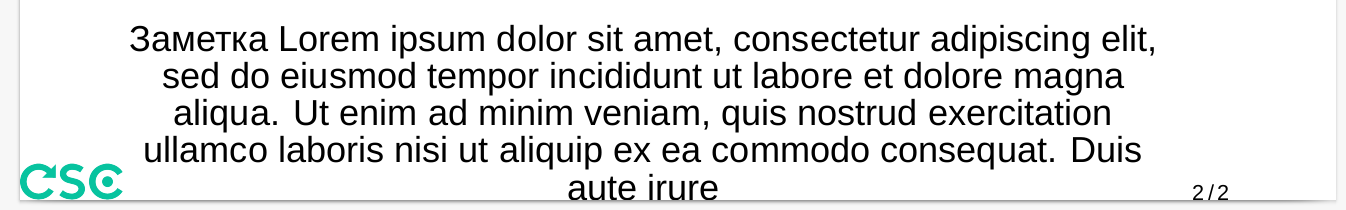
\includegraphics[width=0.7\textwidth]{06_box.png}\par}
\pause
\begin{itemize}
    \item \TeX-путь: 
    \begin{enumerate}
        \item Обернём все элементы в боксы 
        \item Ограничим ширину заметки с помощью \ccol\hspace=...
        \item Поднимем заметку выше
    \end{enumerate}
    \item \LaTeX-путь:
    \begin{enumerate}
        \item Обернём все элементы в нужные боксы 
    \end{enumerate}
\end{itemize}
\pause

Вопрос: как сделать, чтобы между элементами было пустое пространство?
}


\begin{frame}{Пробелы}\relax
    {\LARGE \ccol{Клей} и \ccol{Керны} предоставляют пробелы между боксами.}
    \samePosPicture{intro}{11-11}

    \cscfootnote{\tugC{https://www.tug.org/utilities/plain/cseq.html\#kern-rp} \knuthc{12}[79]}
\end{frame}

\begin{frame}[fragile]{Что такое клей}\relax
    Но клей -- это больше, чем просто ``пробел'' между боксами.
    
    Клей это {\bfseries \ccsc растяжимый} пробел между боксами.
    
    \inpause
    %      \lstset
    % {
    %     basicstyle=\tt\normalsize,
    % }
    \footnotesize
        \begin{tabbing}
     
        \lstinline|\hskip |\= \lstinline|2em | \= \lstinline|plus 0.5em | \= \lstinline|minus 0.6em|\kill

        \rulecommand{1}\lstinline|\hskip |\> \rulecommand{2}\lstinline|2em | \> \rulecommand{3}\lstinline|plus 0.5em | \> \rulecommand{4}\lstinline|minus 0.6em| \\ \footnotesize
        добавить горизонтальный клей (\TeX). \ccol\vskip\ добавит вертикальный\>  \> \>  \\ 
        \>\footnotesize базовый отступ  \> \> \\ 
        \>  \>\footnotesize насколько может растянуться (опционно)  \> \\
        \>  \> \> \footnotesize насколько может сужаться (опционно) \\
        
    \end{tabbing}
    
    \begin{tabbing}
     
        \lstinline|\hspace{|\= \lstinline|2em | \= \lstinline|plus 0.5em | \= \lstinline|minus 0.6em}|\kill

        \rulecommand{1}\lstinline|\hspace{|\> \lstinline|2em | \> \lstinline|plus 0.5em| \> \lstinline|minus 0.6em}| \\ \footnotesize
        добавить горизонтальный клей (\LaTeX). \ccol\vspace\ добавит вертикальный.\>  \> \>  \\         
    \end{tabbing}
    \cscfootnote{\tugC{https://www.tug.org/utilities/plain/cseq.html\#hskip-rp} \tugC{https://www.tug.org/utilities/plain/cseq.html\#vskip-rp} \lmanc{19.2}[167] \lmanc{19.14}[176]\\ 
        ещё есть \ccol{\vspace*} -- добавит вертикальный клей в начале страницы
    }
     
\end{frame}


\begin{frame}{Где клей добавляется неявно}\relax
    \obeylines
    \hbox spread -10pt {Между словами и предложениями. Тут много клея.}
    \hbox spread -5pt  {Между словами и предложениями. Тут много клея.}
    \hbox              {Между словами и предложениями. Тут много клея.}
    \hbox spread 5pt   {Между словами и предложениями. Тут много клея.}
    \hbox spread 10pt  {Между словами и предложениями. Тут много клея.}
    \hbox spread 20pt  {Между словами и предложениями. Тут много клея.}
    \hbox spread 40pt  {Между словами и предложениями. Тут много клея.}

    \outclasshigh{\small P.S. Тут \string\hbox\ растянутый в диапазоне -10pt---40pt. Заметьте, что между предложениями растяжение больше, чем между словами. И что дефолтное растяжение -- третья строка -- не минимально.

    А ещё клей есть между параграфами.}
\end{frame}

\begin{frame}{Бесконечный клей}\relax\vspace*{-3ex}
     \lstset
    {
        basicstyle=\tt\tiny,
    }
    \samePosPicture{fillmy}{11-16} 
     
    \ccol{fil}, \ccol{fill}, \ccol{filll} добавляют бесконечность разной ``степени''
    
    \cscfootnote{\knuthc{12}[83] }
\end{frame}

\begin{frame}{Аббревиатуры}\relax
     Можно использовать:
     
     \ccol\hfil \hfill \ccol\hfill \hfill \ccol\hspace\{\ccol\fil\} \hfill  \ccol\hspace\{\ccol\fill\}
     
     \ccol\vfil  \hfill \ccol\vfill  \hfill \ccol\vspace\{\ccol\fil\} \hfill  \ccol\vspace\{\ccol\fill\}
     
     \ccol\hss, \ccol\vss\ -- бесконечный клей как в \textit{plus} так и в \textit{minus}.
\end{frame}

\lookCode{Добавим бесконечный клей между элементами

{\centering
\includegraphics[width=0.7\textwidth]{07_glue.png}\par}\pause

\begin{enumerate}
    \item Добавим \ccol\hfill между лого и заметкой, между заметкой и номером слайда
    \item Добавим немного вертикального клея, чтобы отодвинуть текст от нижнего края 
    \item Добавим немного горизонтального клея перед лого, чтобы отодвинуть его от левого края 
     
\end{enumerate}
}
\lookCode{И давайте изменим отображение заголовка

{\centering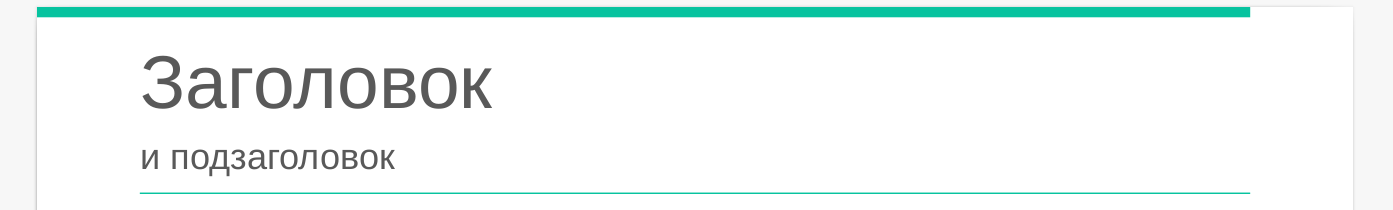
\includegraphics[width=0.7\textwidth]{07_glue2.png}\par}

\pause
\begin{enumerate}
    \item Модифицируем \texttt{frametitle}
    \item Добавим заголовок \ccol\insertframetitle, подзаголовок \ccol\insertframesubtitle
    \item Проведём черту под подзаголовком, чтобы отделить его зрительно \ccol\rule
     
\end{enumerate}
\pause


Проблема: плохо, что чёрточка под заголовком не прижимается к нему, когда нет подзаголовка}
% %%%%%%%%%%%%%%%%%%%%%%%%%%%%%%%%%%%%%%%%%%%%%%% МОДЫ И ПАРАГРАФЫ %%%%%%%%%%%%%%%%%%%%%%%
\subsection{Моды и создание параграфов}
\begin{frame}{Моды\magicPage}\relax
\small
\TeX\ имеет 3(6) мод:
\footnotesize
\begin{enumerate}
    \item {\bfseries {\ccsc Vertical} mode.} [Создание главного вертикального списка, из которого получаются страницы.]
\item {\bfseries Internal {\ccsc vertical} mode.} [Вертикальный список для vbox.]
\item {\bfseries {\ccsc Horizontal} mode.} [Создание горизонтального списка для параграфов.]
\item {\bfseries Restricted {\ccsc horizontal} mode.} [Создание горизонтального списка для hbox.]
\item {\bfseries {\ccsc Math} mode.} [Создание математической формулы внутри горизонтального списка.]
\item {\bfseries Display {\ccsc math} mode.} [Создание математической формулы и положение её на отдельную строку, прерывание параграфа.]
     
\end{enumerate}
     
     \cscfootnote{\knuthc{13}[95]}
\end{frame}

\begin{frame}{Разница между модами\magicPage}

    Много мелких различий. Например:
    \begin{itemize}
        \item в горизонтальной моде только первый пробел имеет значение
        \item в математической моде шрифт по умолчанию - италик, пробелы игнорируются
        \item в выделенной математической моде операторы рисуется больше, чем в обычной
        \item в вертикальной моде все пробелы и <return>ы игнорируется
         
    \end{itemize}
     \cscfootnote{можно использовать \ccol\leavevmode\ чтобы прерывать вертикальную моду}
\end{frame}

\outclassframe{
\begin{frame}{Ещё чуть-чуть о математической моде}
    В реальности у нас есть 4 стиля:\small
     
     \centering 
     \begin{tabular}{l|l|l|p{7em}}
     \hline
     \footnotesize Display style &\footnotesize \ccol\displaystyle & $\displaystyle A$ &\scriptsize главный стиль для выделенной формулы\\
     \footnotesize Text style & \footnotesize\ccol\textstyle & $\textstyle A$ & \scriptsize главный стиль для внутритекстовой формулы\\
     \footnotesize Script style & \footnotesize\ccol\scriptstyle & $\scriptstyle A$ & \scriptsize главный стиль для индексов\\
     \footnotesize Script-script style & \footnotesize\ccol\scriptscriptstyle & $\scriptscriptstyle A$ & \scriptsize главный стиль для под-индексов\\
     \end{tabular}
     
    \cscfootnote{\knuthc{17}[151]}
\end{frame}
}

\begin{frame}{Создание параграфов}{Для перфекционистов}\relax
     \centering
    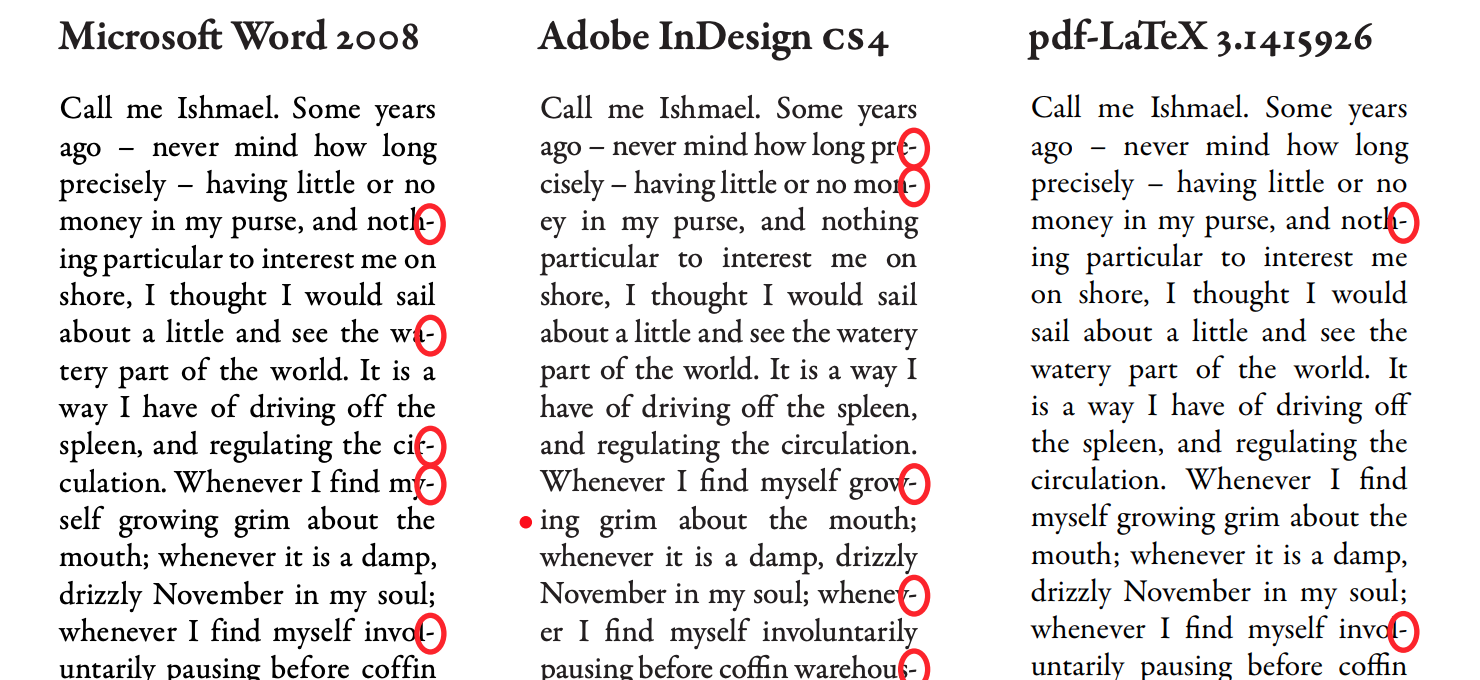
\includegraphics[width=0.6\textwidth]{twcomp}
    
    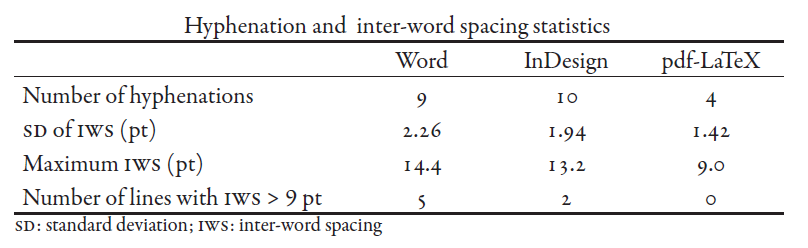
\includegraphics[width=0.6\textwidth]{twcomp2}
    
    \cscfootnote{\stExC{https://tex.stackexchange.com/questions/110133/visual-comparison-between-latex-and-word-output-hyphenation-typesetting-ligat} \url{http://www.rtznet.nl/zink/latex.php?lang=en}}
\end{frame}

\begin{frame}{Создание параграфов}\relax\magicPage
    \Huge\centering ``это, по факту, наверно самый интересный аспект всей системы TEX''\\\hfill \large D. Knuth, the \TeX Book

\end{frame}

\inclassframe{
\begin{frame}{Создание параграфов}
\Large ... но посмотрите его дома :)
\end{frame}
}

\cprotect\outclassframe{
\begin{frame}{Обзор}\relax
    \begin{itemize}
        \item Каждый параграф создаётся целиком: слова в конце параграфа могут повлиять на расположение строк в начале.
        \item \TeX\ никогда не положит слова ближе, чем позволяет клей.
        \item \TeX\ проблует все комбинации разрывов строк. Для каждого варианта и каждой строки \TeX\ вычисляет параметр \textit{badness}. Если он меньше \ccol\tolerance, \TeX\ попробует создать параграф с минимальным числом переносов слов.
        \item если у \TeX 'а не получается, он выдаст \textbf{Overfull} или \textbf{Underfull} ворнинги.
    \end{itemize}
    \cscfootnote{\knuthc{14}[101] \lvoc{3.6}[114] \lmanc{9}[100]}
\end{frame}

\begin{frame}[fragile]{Как управлять переносами слов}\relax

    Локально: использовать \ccol\- ~ \verb|as in this ve\-ry long se\-nta\-nce|
    
    Глобально: \ccol\hyphenation\verb|{some-thing poss-ible}|
    
    \cprotect\cscfootnote{\vspace{-3ex}\ccol\- это короткая версия для команды \ccol\discretionary\verb|{hpre-break texti}{hpost-break texti}{hno-break texti}|\\ 
    так же: \TeX\ никогда не перенесёт слово с ``/''. используйте вместо этого \ccol\slash, если перенос нужен. А \ccol\uchyph=0 запретит перенос слов с Большой буквы.}
\end{frame}

\begin{frame}{Управление разрывом строк вручную}\relax

    Никогда не прерываются: неразрывный пробел \~, \ccol\nobreak, \ccol\nolinebreak
    
    Всегда: \ccol\\, \ccol\break, \ccol\linebreak
    
    Ещё можно использовать \ccol\obeylines\ И тогда разрывы будут происходить там же, где в исходном коде.
     
     \cscfootnote{кстати: \ccol\\ \ имеет опционный параметр: вертикальный отступ после себя. А \ccol\smallskipamount, \ccol\medskipamount\ и \ccol\bigskipamount\ отвечают за разрыв после параграфа. \ccol\linebreak\ имеет опционный параметр: [0-4] насколько сильно ваше желание прервать строку после этого.}
\end{frame}

\begin{frame}{Алгоритм: часть 1}\relax

    \begin{enumerate}
        \item \TeX\ создаёт варианты без переноса слов. Проверяет параметр \textit{badness} с параметром \ccol\pretolerance. 
        \item \textit{badness} $\simeq$ 100$\cdot$<proportion-between-the-normal-glue-and-its-stretching/compression>$^3$
        \item если проверка с \ccol\pretolerance\ провалилась, \TeX\ попробует все комбинации разрывов строк, чтобы badness была меньше, чем \ccol\tolerance
         
    \end{enumerate}
     
     \cscfootnote{Умолчания: \ccol\pretolerance=100, \ccol\tolerance=200}
\end{frame}

\begin{frame}{Алгоритм: часть 2}\relax
    \footnotesize
    \begin{enumerate}
        \item разрывы строк допустимы лишь в следующих местах:
        \begin{enumerate}
            \item клей
            \item керн, после которого идёт клей 
            \item математика (\$) с последующим клеем
            \item ручное или автоматическое прохождение штрафа
            \item  discretionary разрыва
        \end{enumerate}
        \item Пенальти для клея -- $0$. Для разрыва это \ccol\hyphenpenalty=\ или \ccol\exhyphenpenalty=. Пенальти можно добавить вручную через \ccol\penalty
        \item Пенальти может быть как положительная, так и отрицательная. Если оно $>10^4$ тут никогда не будет разрыва, а если $<-10^4$ разрывы будут всегда
         
    \end{enumerate}
         
    \cscfootnote{умолчания: \ccol\hyphenpenalty=50, \ccol\exhyphenpenalty=50\\ 
    а ещё можно добавлять доп пространства между текстом и математикой с \ccol\mathsurround}
\end{frame}


\begin{frame}{Алгоритм: часть 3}\relax

    \begin{enumerate}
    \item В реальности, \TeX\ пытается минимизировать \textit{demerits}. Он пропорциональен {\ccsc badnesses}, \ccol\linepenalty\ (определяет, насколько сильно вы просите \TeX\ уменьшить число строк) и {\ccsc penalty}
    \item \TeX\ так же берёт в расчёт и добавляет пенальти, если две строки подряд имеют перенос слов (\ccol\doublehyphendemerits), и если строки \textit{визуально несовместимы} (например: растянутая линия с ужатой) (\ccol\adjdemerits) и если предпоследняя строка абзаца заканчивается discretionary (\ccol\finalhyphendemerits)
    
    \end{enumerate}
     
     \cscfootnote{Умолчания: \ccol\linepenalty=10, \ccol\adjdemerits=10000, \ccol\doublehyphendemerits=10000, \ccol\finalhyphendemerits=5000.\\ 
     \ccol\hfuzz=... добавит максимальную длину выравнивания строки}
\end{frame}

\begin{frame}{Что ещё }\relax 
    \def\strutdepth{\dp\strutbox}
    \def\marginalstar{\strut\vadjust{\kern-\strutdepth\specialstar}}
    \def\specialstar{\vtop to \strutdepth{
    \baselineskip\strutdepth
    \vss\llap{* }\null}}
    
    \begin{itemize}
        \item Используйте \ccol\narrow\ чтобы сузить строки
        \item \ccol\looseness=-1 чтобы попросить \TeX\ попробовать уменьшить число строк в параграфе
        \item \ccol\prevgraf\ показывает текущую строку параграфа
        \item \ccol\vadjust\ добавляет что-то в вертикальный список после каждого параграфа. Например, так мы добавили звёздочку слева \marginalstar
        \item \ccol\everypar\ добавляет что-то после каждого параграфа
        \item \ccol\parfillskip\ --- клей после каждой строки
        \item \ccol\parskip\ --- вертикальный клей между параграфами
         
    \end{itemize}
     
\end{frame}

\begin{frame}{Создание страниц}\relax
    \begin{itemize}
        \item Кнут создал \TeX\ тогда, когда памяти оптимизировать всю страницу ещё не хватало.
        \item \TeX\ ищет лучший разрыв для текущей страницы и удаляет страницу из памяти.
        \item В целом алгоритм примерно такой же.
        \item Можно использовать \ccol\penalty\ or \ccol\nobreak\ в вертикальном моде
        \item Можно использовать \raggedbottom\ чтобы убрать привязку вертикальную к низу страницы
        \item По аналогии с параграфами, можно использовать \ccol\newpage, \ccol\pagebreak, \ccol\nopagebreak
         
    \end{itemize}
     
     \cscfootnote{\knuthc{15}[119] \lvoc{III.9}[141] \lmanc{10}[105]}
\end{frame}
}
%%%%%%%%%%%%%%%%%%%%%%% Передача параметров, опционные аргументы %%%%%%%%%%%%%%%%
\subsection{Возможности создания команд и передачи параметров в \LaTeX}

\begin{frame}[fragile]{Опционные аргументы в создании команд\magicPage }\relax
    \footnotesize
     \begin{tabbing}
     
        \lstinline|\newcommand{\test}|\= \lstinline|[2]| \= \lstinline|[my default arg]| \= \lstinline|{имеет умолчание #1, задаётся #2}|\kill

        \lstinline|\newcommand{\test}|\> \rulecommand{1}\lstinline|[2]| \> \rulecommand{2}\lstinline|[my default arg]| \> \lstinline|{имеет умолчание #1, задаётся #2}| \\ \footnotesize
        \>\footnotesize общее число аргументов  \> \> \\ 
        \>  \>\footnotesize какие аргументы по умолчанию \> \\
        \> \>~~~~(по порядку с начала) \>
    \end{tabbing}
    
    \vspace{-3ex}
    \lstinline|\usepackage{xargs}|\\ 
    \lstinline|\newcommandx {\ testOpt }[3][3= def opt val]|
    
    Для именнованных команд можно использовать пакет \textit{keyval} или \textit{pgfkeys}
    
    \cscfootnote{\stExC{https://tex.stackexchange.com/questions/58069/newcommand-key-value} \stExC{https://tex.stackexchange.com/questions/34312/how-to-create-a-command-with-key-values} \stExC{https://tex.stackexchange.com/questions/26771/a-big-list-of-every-keyval-package}}
     
\end{frame}

\begin{frame}[fragile]{Передача параметров в пакет}\relax
    \footnotesize
    \lstinline|\RequirePackage{kvoptions}| -- используем пакет \\ 
    \lstinline|\SetupKeyvalOptions{family=KVCSC, prefix=KVCSC@}| -- задаём namespace. Теперь параметр {\ccsc foobar} будет доступен как \ccol{\KVCSC@foobar}
    \vspace{-1ex}
    {\scriptsize
    \lstset{basicstyle=\tt\tiny}
    \begin{tabbing}
     
     \lstinline|\DeclareStringOption|\= \lstinline|[noarg]| \= \lstinline|{argname}| \= \lstinline|[default arg value]|\kill

        \lstset{basicstyle=\tt\tiny}\lstinline|\DeclareStringOption|\> \rulecommand[10pt]{1}\lstinline|[noarg]| \> \rulecommand[10pt]{2}\lstinline|{argname}| \> \rulecommand[10pt]{4}\lstinline|[default arg value]| \\ 
        \> значение, если аргумент не передан совсем \lstinline|\usepackage{mypackage}|  \> \> \\
        \>  \> имя аргумента для передачи, может быть использована как  \> \\
        \>  \> ~~~~~~~~~~~~~~~~~~~~~~~~~~ \lstinline|\usepackage[myarg=smth]{mypackage}|  \> \\
        \>  \>  \> дефолтный аргумент в случае, если пакет вызывает-  \\
        \>  \>  \> ~~~~~~~~ся как \lstinline|\usepackage[smth]{mypackage}|  \\
    \end{tabbing}
    }

    \vspace{-2ex}
    \lstinline|\ProcessKeyvalOptions*| -- непосредственно подставляем полученные значения
    
    % \lstinline|\KVCSC@argname| -- под таким именем аргумент будет доступен в командах
\end{frame}
\lookCode{Реализуем возможность менять логотип через параметр пакета\pause

\begin{enumerate}
    \item Перенесём новый файл логотипа в рабочую папку
    \item Подключим пакет
    \item Создадим опцию {\ccsc logo}
    \item Передадим эту опцию \ccol{\KVCSC@logo} в создание команды \ccol\logoname
\end{enumerate}}

\inclassframe{
\begin{frame}{За эту часть мы узнали}\relax
    \begin{itemize}
        \item Как создавать стилевые файлы
        \item Как сделать футлайн и заголовок
        \item Как работать с боксами
        \item Как добавить клей
        \item Как создавать команды и передавать параметры в пакеты
    \end{itemize}
    Фактически мы умеем создать любую картинку\inpause, если она статична
\end{frame}
\begin{frame}{Пока мы не знаем}\relax
    \begin{itemize}
        \item Как убрать номер слайда с титульника
        \item Как пододвинуть чёрточку под заголовком ближе к нему, когда подзаголовка нет
        \item Как делать динамические элементы типа прогрессбара
        \item Как можно манипулировать элементами
    \end{itemize}\inpause
    Т.е. для полноты картины нужно научиться работать с:
    \begin{itemize}
        \item условными операторами
        \item переменными
        \item циклами
    \end{itemize}\inpause
    научиться программировать на \TeX!
\end{frame}
}